\documentclass[output=paper]{langscibook}
\ChapterDOI{10.5281/zenodo.5524274}
\author{Emily A. Hanink\affiliation{The University of Manchester}}
\title{Restructuring and nominalization size}
\abstract{This paper addresses the interaction between restructuring and nominalization in Washo (isolate, USA). An overview of the basics of restructuring in Washo is provided, and then two types of thematic nominalizations -- subject and object -- are compared with respect to their underlying structure and the availability of restructuring. Particular attention is paid to predictions determining the availability of both functional and lexical restructuring; with specific regard to the latter, the Washo data offer preliminary evidence that the height of the nominalization must contain at least VoiceP to faciliate agent sharing (\citealt{WurmbrandShimamura2017}).}

\begin{document}
\SetupAffiliations{mark style=none}
\tikzset{every tree node/.style={align=center,anchor=north}} 
\maketitle

\section{Introduction}

 This paper addresses the interaction between restructuring and nominalization size in Washo (isolate, USA). While Washo allows for restructuring in some nominalizations, it is shown that sufficient structure must be projected. I demonstrate this with a comparison between two types of thematic nominalizations in the language, subject and object, which differ in their underlying structure. The interaction between restructuring and nominalization is not well-studied, but offers an exciting venue for future research. The modest aim of this paper is therefore to offer some discussion of the  basics of restructuring in Washo (\sectref{haninksec:2}), and to highlight some questions regarding the relationship between nominalization height and the availability of restructuring, based on currently available data (\sectref{haninksec:3}--\sectref{haninksec:4}).

\section{Restructuring in Washo}\label{haninksec:2}


The term {\itshape restructuring} refers to constructions in which an ``embedded predicate is transparent
for properties which are otherwise clause-bound'' \citep[248]{wurmbrand2015}. For example, one common diagnostic for restructuring comes from the availability of clitic climbing, as shown with the Italian contrast in (\ref{haninkitaliana}--\ref{haninkitalianb}) \citep[991--992]{Wurmbrand2004}:

\ea Italian\\
 \ea[]{
  \gll Lo volevo $[$ vedere {\itshape t}$_{\text{cl}}$ subito\ $]$.\\
  him I-wanted {} see {} immediately\\
  \glt `I wanted to see him immediately.' \hfill {\itshape Restructuring}\label{haninkitaliana}
 }
 \ex[*]{
  \gll Lo detesto $[$ vedere {\itshape t}$_{\text{cl}}$ in quello stato\ $]$.\\
  him I-detest {} see {} in that state\\
  \glt Intended: `I detest seeing him in that state' \hfill {\itshape Non-restructuring}\label{haninkitalianb}
 }
 \z
\z
 
 While restructuring phenomenena have largely been studied in analytic-type languages, agglutinative-type languages likewise display restructuring effects. This is  illustrated for example in (\ref{haninkjapanese}) with Japanese, in which the restructuring verb {\itshape wasure} `forget' occurs as as an affix on the non-finite verb {\itshape tabe} `eat' within the same predicate. Such predicates instantiate restructuring in that they exhibit monoclausal effects; see \citealt{shimamurawurmbrand2014} for more details.



\ea Japanese\\
\gll 
 John-wa subete-no ringo-o tabe\textit{-wasure}-ta.\\
John-{\scshape top} all-{\scshape gen} apple-{\scshape acc} eat\textit{-forget}-{\scshape pst}\\
\glt `John forgot to eat all the apples.' \hfill \citep[2]{shimamurawurmbrand2014} \label{haninkjapanese}
\z

 
 In Washo, a head-final language like Japanese, restructuring verbs are likewise affixed onto a non-finite (tenseless) verb to form a complex predicate (\ref{haninkrest}).\footnote{Washo (iso: was) is an endangered isolate spoken in several communities of California and Nevada surrounding Lake Tahoe. Some typologists group Washo within the Hokan family, see e.g., \citet{campbell1997} and \citet{mithun1999} for discussion. Orthography is adapted from \citet{jacobsen1964}; non-IPA symbols in this paper are L [l̥], š [ʃ], and y [j]. Stress is represented with an acute accent. Unless otherwise stated, the Washo data come from the author's fieldwork.} 
 
 \ea\label{haninkrest} Washo\\
 \gll l-éšɨm\textit{-dugá:gu}-yi\\
1-sing\textit{-not.know.how}-\textsc{ind}\\ 
\glt `I don't know how to sing.'\footnote{Some verbs in Washo are inherently negative, as is the case with {\itshape dugá:gu} `not know how'.} 
\z 
 
\noindent Here, clause-bound transparency is revealed by the presence of a single agreement morpheme at the left periphery (prefixal agreement is only for person). Agreement morphology may not appear on both verbs, which I take as evidence for the reduced and non-finite status of the embedded verbal domain. In the same vein, just one set of TAM marking is observed at the right periphery;  negation must likewise be clause-peripheral, and may not intervene between the verbs.


This strategy stands in contrast for example to finite embedding in the language, which comes in the form of either a clausal nominalization  (\ref{haninkadele}) or a bare (non-nominalized) clause (\ref{haninkdream}), depending on the embedding predicate (\citealt{haninkbochnak2018}). Independent tense and mood marking are permitted in both of these clause types.\footnote{Washo is an optional tense language (\citealt{bochnak2016}), and tense marking often does not appear.}  Clausal nominalizations further provide evidence for a CP-layer in that they exhibit switch reference morphology (see \citealt{arregihanink2018}). The upshot is that both of these embedding strategies involve finite clauses.

\ea Finite embedding of a clausal nominalization (nominalized CP)\label{haninkadele}\\
\gll Adele $[$ \textit{pro} daláʔak ʔ-í:gi\textit{-yi-$\varnothing$}-ge $]$ hámup'a-yé:s-i\\
Adele $[$ \textit{pro} mountain 3/3-see-\textit{\textsc{ind-ss}}\textsc{-nm.acc} $]$ 3/3.forget-\textsc{neg-ind}\\
\glt`Adele remembers that she saw the mountain.'\footnote{`Remember' in Washo can only be expressed by negating `forget'.}
\ex Finite embedding of a bare clause (MoodP)\label{haninkdream}\\
\gll \textit{pro} $[$ \textit{pro} di-yé-{iʔ}iš{\itshape-aʔ} $]$ di-gum-su{ʔ}ú{ʔ}uš-i{ʔ}-i \\
 \textit{pro} $[$ \textit{pro} 1-fly-forward\textit{-\textsc{dep}} $]$ 1-\textsc{refl}-dream-\textsc{attr-ind}\\
\glt `I dreamt that I was flying.' \hfill Washo Archive
\z

\subsection{Restructuring in Washo}
Restructuring in Washo is found with a range of aspectual suffixes (\ref{haninkaspect}), as well as with modal `know how to' (\ref{haninkmodal}) and  desiderative `want' (\ref{haninkwant}) (which can also mean `like'). Below I have classified a subset of these verbs (a term used loosely here, see \sectref{haninksec:vs}) based on Grano's (\citeyear{grano2012diss}: 16) sorting of Landau's (\citeyear{landau2000}) classes; Grano draws from the set of restructuring verbs in \citet[342]{wurmbrand2001}. The examples in (\ref{haninkother}) list some verbs in Washo that do not fall clearly into any of these categories.


\ea Aspectual\label{haninkaspect}\\
\ea {\gll zí:gɨn l-éʔw\textit{-gáŋa}-leg-i\\
chicken 1/3-eat\textit{-start}-{\scshape rec.pst-ind}\\
\glt `I started to eat the chicken.' \hfill Washo Archive}
\ex mí:-lé:we di-dulé:k'ɨl\textit{-mámaʔ}-ášaʔ-i\\
2.{\scshape pro}-for 1-cook\textit{-finish}-{\scshape prosp-ind}\\
\glt `I'll finish cooking for you.' 
\ex \gll háʔaš\textit{-dúweʔ}-i\\
3.rain\textit{-be.about.to}-{\scshape ind}\\
\glt `It's about to rain.'\label{haninkrain}
\ex \label{haninksmoke}\gll t'é:liwhu báŋkuš\textit{-íweʔ}-i\\
 man 3.smoke-stop-{\scshape ind}\\
\glt `The man stopped smoking.' \hfill Washo Archive
\z
\ex Modal\\
{\gll t'é:liwhu bašáʔ\textit{-dugá:gu}-yi\\
 man 3.write\textit{-not.know.how}-{\scshape ind}\\
\glt `The man doesn't know how to write.'} \label{haninkmodal}
\ex Desiderative\label{haninkwant}\\
\ea {\gll di-gé:gel\textit{-gaʔlám}-i\\
1-sit\textit{-want}-{\scshape ind}\\
\glt `I want to sit.'\hfill Washo Archive} 
\ex  \gll l-éšɨm\textit{-gaʔlám}-i\\
1-sing\textit{-like}-{\scshape ind}\\
\glt `I like to sing.'
\z 
\ex Other\label{haninkother} 
\ea \gll di-bamušéʔeš\textit{-tamugáyʔliʔ}-i\\
1-read\textit{-be.tired.of}-{\scshape ind}\\
\glt `I'm tired of reading.'
\ex \gll l-éšɨm\textit{-duwéʔweʔ}-ášaʔ-i\\
1-sing\textit{-try}-{\scshape prosp-ind}\\
\glt `I'm going to try to sing.'\footnote{The verb `try' is the reduplicated from of the aspectual verb `be about to' (\ref{haninkrain}). This is an unusual instance of reduplication, which generally indicates plurality in Washo (see \citealt{yu2005,yu2012}).}
\ex \gll di-gum-yá:gɨm\textit{-ŋáŋa}-hu-yaʔ\\
1-{\scshape refl}-smoke\textit{-pretend}-{\scshape pl.incl-dep}\\
\glt `Let's pretend to smoke one another.' \hfill Bear and Deer Story
\z 
\z 

\subsection{Lexical vs. functional restructuring} \label{haninksec:vs}\largerpage[1.75]
\citet{wurmbrand2001} argues for a distinction between {\itshape lexical} and {\itshape functional} restructuring (see also \citealt{Wurmbrand2004}; cf. \citealt{cinque2001,cinque2004,grano2012diss}), which depends on  whether the restructuring element is a lexical verb or a functional head, e.g., Asp or Mod. I show in this section that this distinction, which will come up in the discussion of nominalizations, appears to be  motivated in Washo. 

\citet{Wurmbrand2004} lays out several diagnostics for lexical vs. functional restructuring. For example, only lexical restructuring verbs show flexibility in selection. In Washo, this is observed in that lexical verbs may select for a nominal argument (\ref{haninkshoes}); this is however not possible in functional restructuring (\ref{haninkbook}).

\ea Variation in selection
\ea[] {\gll $[$ di-mók'o $]$ di\textit{-tamugáyʔliʔ}-i\\
$[$ 1-shoe $]$ 1/3\textit{-be.tired.of}-{\scshape ind}\\
\glt `I'm tired of my shoes.'\label{haninkshoes}}
\ex[*] {\gll $[$ ʔitbamušéʔeš $]$ di\textit{-gáŋaʔ}-i\\
$[$ book $]$ 1/3\textit{-start}-{\scshape ind}\\
\glt Intended: `I started the book.'\label{haninkbook} }
\z
\z

\begin{sloppypar}Second, functional restructuring is compatible with weather subjects (\ref{haninkstopcold}), while lexical restructuring is not (\ref{haninktiredcold}):\end{sloppypar}

\ea Weather verbs
\ea[*] {\gll baŋáya wa-métuʔ\textit{-tamugáyʔliʔ}-i\\
outside {\scshape stat}-be.cold{\itshape -be.tired.of}{\scshape -ind}\\
\glt Intended: `It's tired of being cold outside.'\label{haninktiredcold}}
\ex[] {\gll baŋáya wa-métuʔ\textit{-iweʔ}-i\\
outside {\scshape stat}-be.cold{\itshape -stop}{\scshape -ind}\\
\glt `It stopped being cold outside.'\label{haninkstopcold}}
\z
\z

Additionally, Washo exhibits cross-linguistically rare object control in restructuring (cf. \citealt{cinque2001}), exemplified in (\ref{haninkobjectcontrol}) with the verb {\itshape méwɨl} (`ask (someone) to do something'). Such examples pose a problem for accounts in which restructuring is limited entirely to functional heads, as such heads are predicted not to be able to select for internal arguments.

\ea
\gll Adele l-é:biʔ{\itshape -méwɨl}-i\\
Adele 1/3-come{\itshape -ask}-{\scshape ind}\\
\glt `I asked Adele to come.' \label{haninkobjectcontrol}
\z 


Finally, variation is observed in possible orderings of the causative morpheme. In cases of lexical restructuring, the causative morpheme may appear as a suffix on the lower verb (\ref{hanink1}), or at the periphery of both verbs (\ref{hanink2}).\footnote{This may in fact be a diagnostic for the optionality of lexical restructuring.} In cases of functional restructuring, it may only appear in a right-peripheral position (\ref{haninkfunccaus}).\footnote{The position of the causative morpheme in Washo is sensitive to phonological factors, see e.g.,  \citealt{jacobsen1973,benz2018}, but that is not what is driving the contrast here.} 

\ea Position of the causative in lexical restructuring
\ea \gll dímeʔ di-yák'aš{\itshape-ha}-gaʔlám-i\\
water 1/3-be.warm-\textit{\textsc{caus}}-want{\scshape-ind}\\
\glt `I want to warm the water up.' \label{hanink1}
\ex \gll dímeʔ di-yák'aš-gaʔlám{\itshape -ha}-yi\\
water 1/3-be.warm-want\textit{\textsc{-caus}}{\scshape-ind}\\
\glt `I want to warm up the water.' \label{hanink2}
\z
\ex Position of the causative in functional restructuring\label{haninkfunccaus}
\ea[]{ \gll dímeʔ di-yák'aš-gáŋa{\itshape-ha}-yi\\
water 1/3-be.warm-start\textit{\textsc{-caus}}{\scshape-ind}\\
\glt `I'm starting to warm the water up.' \label{hanink3}}
\ex[*] {\gll dímeʔ di-yák'aš{\itshape-ha}-gáŋaʔ-i \\
water 1/3-be.warm-\textit{\textsc{caus}}-start-{\scshape ind}\\
\glt Intended: `I'm starting to warm the water up.' \label{hanink4}  }
\z
\z



While a precise analysis explaining the range of such effects awaits future research, moving forward I follow \citeauthor{wurmbrand2001} (\citeyear{wurmbrand2001}, et seq.) in treating functional restructuring as involving functional heads in the clausal spine such as Asp/Mod (\citealt{cinque2001,cinque2004,grano2012diss}), represented in (\ref{haninkvoice}) below as ``F'', but lexical restructuring as involving lexical verbs that select for an embedded VoiceP (\ref{haninkvoice2}), in a way to be made more precise in the next subsection.


\begin{multicols}{2}\raggedcolumns
 \ea Functional restructuring\label{haninkvoice}\\
\begin{tikzpicture}[baseline]
\tikzset{level distance=22pt,sibling distance=15pt}
%\tikzset{level 1/.style={sibling distance=-125pt}}
 \Tree [.FP [.VoiceP \qroof{\dots}.vP [.Voice ] ] [.F ] ] 
  \end{tikzpicture}
\z\columnbreak
 \ea Lexical restructuring\label{haninkvoice2}\\
\begin{tikzpicture}[baseline]
\tikzset{level distance=22pt,sibling distance=15pt}
%\tikzset{level 1/.style={sibling distance=-125pt}}
 \Tree [.VP [.VoiceP \qroof{\dots}.vP [.Voice ] ] [.V ] ] 
  \end{tikzpicture}
\z 
\end{multicols}

\subsection{Lexical restructuring involves agent sharing}\label{haninksec:agent}

Relevant for the discussion of nominalizations moving forward is the proposal that lexical restructuring involves the selection of VoiceP by a restructuring verb (\citealt{wurmbrand2015,WurmbrandShimamura2017}), rather than the selection of a bare VP (e.g., \citealt{wurmbrand2001,Wurmbrand2004}).
This proposal is motivated by languages that show a variety of effects of Voice in restructuring enivronments.\footnote{While voice distinctions play a large role here, Washo lacks a passive (\citealt{jacobsen1979}).} I briefly summarize their approach and show how it extends to Washo. 

Adopting the proposal that (causative) $v$ co-occurs with Voice within a split-voice domain (i.a. \citealt{bowers2002,folliharley2005,alexiadouetal2006,marantz2008}),  \citet{WurmbrandShimamura2017} offer the following derivation of a matrix clause with active voice (\figref{haninkvoice3}). In this structure, the Voice head introduces the agent and bears both agent and accusative case features, while v carries transitivity information. The valuation of interpretable $\varphi$-features as well as feature sharing between the DP argument and Voice corresponds to theta-assignment.
 
\begin{figure}
\caption{\label{haninkvoice3}Feature sharing between DP and Voice \citep{WurmbrandShimamura2017}}
\begin{tikzpicture}[baseline]
\tikzset{level distance=22pt,sibling distance=15pt}
%\tikzset{level 1/.style={sibling distance=-125pt}}
 \Tree [.VoiceP \qroof{{\itshape i}$\varphi$: val}.DP  [.Voice$^\prime$ [.Voice\\{\scshape agent, acc}\\{{\itshape i}$\varphi$:\underline{val}} ][.vP [.v\\{\scshape tr/in, (caus)} ] \qroof{$\dots$}.VP ]] ]
 \draw[semithick,dashed,*-*] (-2,-2.25)..controls +(south east:1) and +(south west:1)..(.35,-3.15);
  \end{tikzpicture}
\end{figure}

\citet{WurmbrandShimamura2017}  adopt moreover a valuation approach to Agree (\citealt{pesetskytorrego2007}), formulated in (\ref{haninkreverse}) as Reverse Agree, which accounts for the downward valuation of the agent's features onto Voice.

\ea Reverse Agree \citep{Wurmbrand2014}\label{haninkreverse}\\
A feature {\scshape F}:\underline{\ \ \ } on $\alpha$ is valued by a feature {\scshape f}: val on $\beta$ iff 
\ea $\beta$ c-commands $\alpha$ and
\ex $\alpha$ is {\itshape accessible to $\beta$}
\ex $\alpha$ does not value \{a feature of $\beta$\}/\{a feature {\scshape f} of $\beta$\}
\z
\z


In restructuring configurations (see below), the restructuring verb selects for VoiceP.  Crucially, matrix Voice agrees with the DP subject in its specifier before valuing {\itshape i}$\varphi$ on the lower Voice head (see \citealt{wurmbrand2015,WurmbrandShimamura2017} for distinctions between voice matching and default voice languages). No embedded subject is projected; this proposal therefore accounts for the fact that an overt subject is not allowed in the embedded VoiceP. Instead, feature sharing results in agent sharing between Voice heads. 


Evidence for the presence of embedded VoiceP in Washo  comes from the appearance of the causative morpheme {\itshape -ha} between the lower and higher verbs, indicating that the complement of the restructuring verb is larger than VP. Adopting  Wurmbrand \& Shimamura's (\citeyear{WurmbrandShimamura2017}) proposal for Washo, the structure for an example such as (\ref{haninkwarmup}) is then as in \figref{fig:haninkwarmupstructure} (schematized without head movement). No embedded subject is projected, instead embedded Voice enters into a dependency with the higher Voice head, whose features it then shares.
 
 % (as is also the case in Acehnese, \citealt{legate2014}, apud \citealt{wurmbrandshimamura2017}), 

\ea \label{haninkwarmup}
\gll dímeʔ di-yák'aš-ha-tamugáyʔliʔ-i\\
water 1/3-be.warm-{\scshape caus}-be.tired.of-{\scshape ind}\\
\glt `I'm tired of warming up the water.'
%\gll géwe di-yúli-duwéʔweʔ-ha-yášaʔ-i\\
%coyote 1/3-die-try.{\scshape fut}-{\scshape caus-near.fut-ind}\\
%\glt `I'm going to try to kill the coyote.'
\z


\begin{figure}
\caption{General schematic for restructuring in Washo\label{fig:haninkwarmupstructure}}
\begin{tikzpicture}
\tikzset{level distance=22pt,sibling distance=15pt}
\tikzset{level 1/.style={sibling distance=-125pt}}
\tikzset{level 2/.style={sibling distance=15pt}}
\tikzset{level 3/.style={sibling distance=-10pt}}
\tikzset{level 4/.style={sibling distance=0pt}}
\tikzset{level 5/.style={sibling distance=15pt}}
 \Tree [.VoiceP [.{\itshape pro}\\{i$\varphi$:val} ] [.Voice$^{\prime}$   [.vP [.VP [.VoiceP  [.vP \qroof{\itshape dímeʔ yák'aš}.VP$_2$  [.v\\{\scshape caus}\\{\itshape -ha} ] ] [.Voice\\{i$\varphi$: \underline{val$_{ag}$}} ] ] [.V\\{\itshape -tamugáyʔliʔ}  ] ] [.v ] ]  [.Voice\\{i$\varphi$: val$_{ag}$} ] ] ]
  \draw[semithick,dashed,*-*] (-.5,-5.25)..controls +(south east:1.5) and +(south west:1)..(3.75,-2.65);
  \end{tikzpicture}
%\begin{tikzpicture} 
%\tikzset{level distance=25pt,sibling %distance=20pt}\Tree[.vP [.VP$_1$ [.vP$_R$ \qroof{\itshape %duwéʔweʔ}.VP$_2$  [.$<$v$_R$$>$ ] %] [.V$_1$ [.V$_1$\\{\itshape -yuli} ] [.v$_{R}$\\{\itshape -ha} ] %] ] [.v ] ]  \end{tikzpicture}
\end{figure}



\section{Restructuring in nominalizations}\label{haninksec:3}

I now turn to the interaction between restructuring and nominalization. Beyond the sentential level, restructuring is also observed in certain nominalizations; by contrasting subject and object nominalizations, I show below  that the height of the nominalization determines whether restructuring is possible. Functional restructuring requires higher aspectual heads to be present in order to obtain, while the proposal put forward in \sectref{haninksec:agent} predicts that the projection of at least VoiceP  within the nominalization is required for lexical restructuring. %I show that the availability of restructuring in subject nominalizations is consistent with this prediction.

\subsection{Thematic subject nominalizations}

The first nominalization type I discuss is thematic subject nominalizations, characterized in Washo by a lack of TAM marking as well as the presence of the phonologically conditioned prefix {\itshape t'-/d\textsuperscript{e}-} (\citealt{jacobsen1964}):

\ea Thematic subject nominalizations
\ea \gll{\itshape da}-mt'áʔŋaʔ\\
\textit{\textsc{3.un}}-hunt\\
\glt `hunter' \hfill Washo Archive
\ex \gll dé:guš {\itshape t'}-í:k'eʔ\\
potato \textit{\textsc{3.un}}-grind\\
\glt `potato grinder' ({\itshape man's name}) \hfill \citep[354]{jacobsen1964}
\z
\z

Much focus in the literature on subject nominalizations has focused on {\itshape -er} nominals (\citealt{rappaporthovavlevin1992,bakervinokurova2009,alexiadouschafer2010}), which are generally limited to external arguments cross-lin\-guis\-ti\-cal\-ly (though see \citealt{alexiadouschafer2008,alexiadouschafer2010}), exemplified in (\ref{haninkenglish}):

\ea a dazzled $[$ admir{\itshape -er} of Washington\ $]$  \hfill (\citealt{rappaporthovavlevin1992})\label{haninkenglish}
\z 



\noindent\citet{bakervinokurova2009} argue that other subject nominalizations are distinguishable from {\itshape -er} nominals by the availability of: (i) direct objects and (ii) unaccusative subjects. In their analysis, deverbal -{\itshape er} nominals do not project beyond VP (cf. \citealt{alexiadouschafer2010}), precluding accusative case licensing as well as external arguments in this nominalization type  (-{\itshape er} is a nominal Voice head (cf. \citealt{kratzer1996}), explaining the restriction to external arguments). 

On the first point, (\ref{haninkhealer}) shows that accusative direct objects are licensed in Washo  {\itshape t'-/d\textsuperscript{e}-} nominalizations ({\itshape t'ánu} `people'; note that accusative is unmarked on nouns), while the presence of v and Voice is diagnosed by the availability of the causative suffix {\itshape -ha}. On the second point, unaccusative subjects are also possible (\ref{haninkbroken}), consistent with the fact that the nominalizer does not take the place of an agentive subject, as on Baker \& Vinokurova's \citeyear{bakervinokurova2009} analysis.\footnote{Unaccusativity is diagnosed by the ability to undergo the inchoative/causative alternation.}


\ea \gll t'ánu t'-íšiw-ha\\
person 3.\textsc{un}-get.well-{\scshape caus}\\
\glt `person healer' (Lit. `one who heals people') \label{haninkhealer}
\ex \gll da-gótaʔ\\
\textsc{3.{\scshape un}}-{break}\\
\glt `something that is broken' \label{haninkbroken}
\z 

\noindent Relatedly, evidence for a syntactically-projected subject in VoiceP (beyond accusative licensing) comes from the availability of reflexives (\ref{haninkcall}), for which {\scshape pro} serves as a licit antecedent (cf. \citealt{bakervinokurova2009} on Gĩkũyũ (Bantu)). \il{Gĩkũyũ}

\ea \gll Ramona de{\itshape -gum}-díʔyeʔ L-éʔ-i\\
Ramona {\scshape 3.{\scshape un}}-\textit{\textsc{refl}}-call 1-be-{\scshape ind}\\
\glt `My name is Ramona.' (Lit. `{one who calls herself Ramona}') \label{haninkcall}
\z

Subject nominalizations in Washo are therefore not of the {\itshape -er} type, and, based on the above behaviors from complementation and subject flexibility, can be taken to contain at least VoicePs (cf.  \citealt{bochnaketal2011}). I note moreover that they are in fact even larger, as there is preliminary evidence that aspectual suffixes are also permitted, as in (\ref{haninkalways}), which contains the progressive suffix {\itshape -giš}:%\footnote{See \citealt{bochnak2015sula} for evidence that this is a grammatical aspect morpheme.}

 \ea \gll t'ánu da-báŋkuš-i{\itshape-giš} k'-é{ʔ}-i\\
person {\scshape 3.un}-tobacco-{\scshape attr}\textit{\textsc{-prog}} 3-be-{\scshape ind}\\
\glt `People are always smoking.' (Lit. `{ones who are continually with tobacco}')\label{haninkalways}
\z



I now turn to the predictions for restructuring. Beginning with functional restructuring, the prediction is that at least AspP/ModP must be projected for restructuring to obtain. We saw in (\ref{haninkalways}) that there is in fact evidence for an AspP layer in these nominalizations, leading to the prediction that functional restructuring should be possible. (\ref{haninknotsing}) shows that this prediction is borne out: functional restructuring with e.g., aspectual {\itshape -íwe} `stop' is permitted:


\ea Functional restructuring in subject nominalizations\\
{\gll t'-íšɨm\textit{-íwe}-yé:s\\
{\scshape 3.un}-sing-\textit{stop}-{\scshape neg}\\
\glt `one who doesn't stop singing'} \label{haninknotsing}
\z

The availability of functional restructuring follows straightforwardly from the fact these nominalizations may contain functional layers such as AspP. This is schematized in \figref{haninksubjectfunctional} for the example in (\ref{haninknotsing}) (shown without negation):\footnote{Note that the presence of PossP in these structures is due to the fact that the prefix {\itshape t'-/d\textsuperscript{e}-} is not an invariant nominalizer, but in fact a form of possessor agreement that appears with covert third person possessors. I do not go into this any further here due, but see \citet{hanink2020}.}

\begin{figure}
\caption{Functional restructuring in subject nominalizations\label{haninksubjectfunctional}}
\begin{tikzpicture}[baseline]
\tikzset{level distance=22pt,sibling distance=15pt}
 \Tree [.PossP [.AspP \qroof{{\scshape pro} \itshape íšɨm}.VoiceP [.Asp\\{\itshape -íwe} ] ] [.Poss\\{\itshape t'-} ] ] \node (c) at (-4.5,-1.05) {{\itshape  Height of nominalization $\rightarrow$}};
   \end{tikzpicture}
 \end{figure}
 
Turning to lexical restructuring, the prediction is specific to VoiceP. On the account presented in \sectref{haninksec:agent}, lexical restructuring requires agent sharing across Voice heads; the height of nominalization must therefore be at least VoiceP. We saw above that subject nominalizations do involve VoiceP as well as a projected subject, leading to the prediction that restructuring should be possible. This is again borne out, as demonstrated in (\ref{haninknoteat}) with the lexical verb {\itshape -gaʔlám} `like': 

\ea Lexical restructuring in subject nominalizations\\
\gll t'-émlu\textit{-gaʔlám}-é:s\\
{\scshape 3.un}-eat\textit{-like}-{\scshape neg}\\
\glt `one who doesn't like to eat' \label{haninknoteat}\hfill Washo Archive
\z


\begin{figure}
\caption{Lexical restructuring in subject nominalizations\label{fig:haninksubjectstructure}}
\begin{tikzpicture}
\tikzset{level distance=22pt,sibling distance=15pt}
\tikzset{level 1/.style={sibling distance=-20pt}}
\tikzset{level 2/.style={sibling distance=-50pt}}
\tikzset{level 3/.style={sibling distance=-75pt}}
\tikzset{level 4/.style={sibling distance=15pt}}
\tikzset{level 5/.style={sibling distance=0pt}}
\tikzset{level 6/.style={sibling distance=0pt}}
 \Tree [.PossP [.AspP [.VoiceP [.{\scshape pro} ] [.Voice$^\prime$  [.vP [.VP [.VoiceP   \qroof{\itshape émlu}.vP    [.Voice\\{i$\varphi$:\underline{val$_{\textsc{ag}}$}} ] ] [.V\\{\itshape -gáʔlam}  ] ] [.v ] ]  [.Voice\\{i$\varphi$: val$_{\textsc{ag}}$} ] ] ] [.Asp ]] [.Poss\\{\itshape t'-} ] ]
 \node (c) at (-5.25,-1.05) {{\itshape  Height of nominalization $\rightarrow$}};
   \draw[semithick,dashed,*-*] (-3.35,-6.65)..controls +(south east:1.5) and +(south west:1)..(.75,-4.25);
   \end{tikzpicture}
 \end{figure}

Unlike functional restructuring, lexical restructuring relies on agent sharing. As the nominalization targets (at least) VoiceP, this is possible because the $\varphi$-features on embedded Voice can be valued by the higher Voice head (see \figref{fig:haninksubjectstructure}, cp. \figref{fig:haninkwarmupstructure}).

In sum, that thematic subject nominalizations in Washo support both functional and lexical restructuring is consistent with the fact that their structure is quite large. Note that if  \citet{bakervinokurova2009} are correct that agent nominalizations contain only VP, then restructuring should not be possible in {\itshape -er}-nominals cross-linguistically, as higher functional heads will not be present, nor will agent sharing be possible. Restructuring thus provides a further diagnostic to distinguish between different types of subject nominalizations.
 

\subsection{Unexpressed theme nominalizations}

I now move on from subject nominalizations to a type of {\itshape object} nominalization in Washo, which I term {\itshape unexpressed theme nominalizations}. This class of nominalizations is characterized by the invariant nominalizing prefix {\itshape d-}, as in (\ref{haninkinternal}): 

\ea Unexpressed theme nominalizations\label{haninkinternal}\\
\ea \gll {\itshape d-}íšɨm\\
\textit{\textsc{nmlz}}-sing\\
\glt `song'
\ex \gll {\itshape d-}á:muʔ\\
\textit{\textsc{nmlz}}-wear.dress\\
\glt `dress' 
%\ex \gll {\itshape da-}háʔaš\\
%\textit{\textsc{nmlz}}-rain\\
%\glt `rain'  %\hfill 5-23-19
\z
\z 


This type of nominalization refers to an unexpressed internal argument (essentially a cognate object, cf. \citet{barker1998} on -{\itshape ee} nominalizations), and can only apply to unergative verbs, not transitives or unaccusatives; Washo distinguishes between transitive/intransitive variants for several of these verbs (\ref{haninkeat}), even with object drop (\ref{haninkeating}) but only the intransitive form may be nominalized by {\itshape d-} (\ref{haninkfood}).


\ea Intransitive vs. transitive `eat'\label{haninkeat}
\ea \gll m-émlu-yi\\
2-eat.{\scshape in}-{\scshape ind}\\
\glt `You're eating.'
\ex \gll t'á:daš m-íʔw-i\\
meat 2/3-eat.{\scshape tr}-{\scshape ind}\\
\glt `You're eating meat.'
\ex \gll  m-íʔw-i\\
2/3-eat.{\scshape tr}-{\scshape ind}\\
\glt `You're eating it.' \hfill \citep[149]{jacobsen1979} \label{haninkeating}
\z
\ex Nominalization of intransitive vs. transitive `eat'\label{haninkfood}
\ea \gll {\itshape d-}émlu\\
\textit{\textsc{nmlz}}-eat.{\scshape in}\\
\glt `food'
\ex[*]{\gll {\itshape d}-íʔw\\
\textit{\textsc{nmlz}}-eat.{\scshape tr}\\
\glt Intended: `food' }
\z
\z

It is crucial here that unexpressed theme nominalizations differ from subject nominalizations in that they are deficient in verbal structure and do not license overt arguments. With this in mind, one way of deriving the meaning for this nominalization type is to treat {\itshape d-} as a root-selecting nominalizer that also introduces a theme (\ref{haninkdenoted}). This would rule out categorization of transitive and unaccusative roots by {\itshape d-}, as they are lexically specified as having a theme and are therefore of type \textit{$\langle$e, $\langle$v, t$\rangle$$\rangle$}. The resulting meaning for the nominalization is then the set of individuals that are the themes of  generic eating events, i.e., {\itshape food}.

\ea 
\ea {\denote{$\sqrt{emlu}$}: $\lambda$$e$$_v$$[$eat($e$)$]$}
\ex {\denote{\itshape d-}: $\lambda$$P_{\langle v,t\rangle}$$\lambda$$x_e$.Gen $e$$[$$P$($e$) \& {\scshape theme}($x$)($e$)$]$}\label{haninkdenoted}
\ex {\denote{\itshape d-} (\denote{$\sqrt{emlu}$}): $\lambda$$x_e$.Gen $e$$[$eat($e$) \& {\scshape theme}($x$)($e$)$]$}
\z
\z

\begin{sloppypar}
The treatment of {\itshape d-}nominalizations as root nominalizations rather than nominalizations of some verbal structure is further corroborated by Marantz's (\citeyear{marantz2001}) diagnostics distinguishing {\itshape root-cycle} vs. {\itshape outer-cycle} attachment. For example, merger with a root is not only consistent with idiosyncractic meanings (\ref{haninkwater}), but also implies that the resulting meaning depends on the semantics of the root itself, rather than on argument structure. Given that the argument structure of unergative verbs does not entail a syntactically projected internal argument, the semantics of this nominalization must be sensitive to the meaning of the root instead. 
\end{sloppypar}

\ea \gll {\itshape d-}ímeʔ\\
\textit{\textsc{nmlz}}-drink\\
\glt `water' ({\itshape not} `(a) drink') \label{haninkwater}
\z
I therefore propose that the nominalizations in (\ref{haninkinternal}) have the structure in \figref{haninkdstructure}.

\begin{figure}
\caption{\label{haninkdstructure}Unexpressed theme nominalizations}
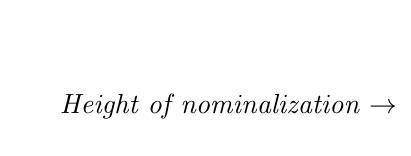
\begin{tikzpicture}[baseline]
\tikzset{level distance=22pt,sibling distance=15pt}
 \Tree [.nP  [.$\sqrt{\textit{emlu}}$ ] [.n\\{\itshape d-} ] ]
  \node (c) at (-3.5,-1) {{\itshape Height of nominalization $\rightarrow$}};
   \end{tikzpicture}
 \end{figure}
 
Relevant for our purposes is that neither functional nor lexical restructuring is ever possible in this type of nominalization (\ref{haninknor}), unlike in the deverbal nominalizations described in the previous subsections.  This fact is immediately obvious if  {\itshape d-}nominalizations are root nominalizations, and therefore do not in fact project any verbal structure (\figref{haninkdstructure}) despite their superficially deverbal appearance.

\ea No restructuring in unexpressed theme nominalizations\label{haninknor}
\ea[*]{\gll d-émlu-gaʔlám\\
\textit{\textsc{nmlz}}-eat.{\scshape in}-like\\
\glt Intended: `food that is liked/wanted'}
\ex[*]{ \gll d-émlu-mámaʔ\\
\textit{\textsc{nmlz}}-eat-finish\\
\glt Intended: `finished food' }
\z
\z
 
To summarize, unexpressed theme nominalizations do not permit restructuring, which is immediately predicted due to their lack of verbal structure. This is of course not surprising, given that they turn out to be root nominalizations. While both subject and object nominalizations superficially appear to be deverbal, the availability of restructuring in the former but not the latter corroborates independently observed differences in the amount of structure they project.

\section{Other nominalizations in Washo} \label{haninksec:4}

We have seen in the previous section that subject nominalizations in Washo are large enough to allow for restructuring, while object nominalizations are not. Before concluding, I turn briefly to two further types of nominalizations in Washo~-- gerunds and instrumental nominalizations -- that lead to predictions about the availability of restructuring, but for which relevant data is lacking at this time.

\subsection{Gerunds}\largerpage

Gerunds in Washo, like subject nominalizations,  lack TAM marking and do not make use of an overt nominalizer. Unlike subject nominalizations however, gerunds allow overt subjects and therefore show normal prefixal agreement, which I again treat as possessor agreement resulting from the presence of Poss (I return to this below).\footnote{Washo exhibits portmanteau agreement marking for subject/object (\citealt{jacobsen1964}), which in this case can be understood as possessor/possessum.} One  environment that gerunds occur in is as the subject of the underspecified modal {\itshape éʔ} (\ref{haninkgive}), which is otherwise a copula (\citealt{bochnak2015wscla,bochnak2015nels}). Another is as the  complement of certain  verbs, e.g., `want' (\ref{haninksleep}).
 
 \ea Gerunds \label{haninkgerunds}
 \ea \gll $[$ hútiweʔ lem-íšɨl $]$ k'-éʔ-i\\
$[$ something  2/1-give $]$ 3-be-{\scshape ind}\\
\glt `You have to give me something.' \\ (Lit. `{Your giving me something is necessary}.') \label{haninkgive}
 \ex \gll $[$ l-élšɨm $]$ di-gaʔlám-i\\
$[$ 1-sleep $]$ 1/3-want-{\scshape ind}\\
\glt `I want to sleep.' (Lit. `{I want my sleeping}.')\label{haninksleep}
 \z
 \z 
 
Based on this distribution, I treat this construction as a type of -{\itshape ing} nominalization. Within the domain of {\itshape ing}-nominalizations, \citet{kratzer1996} distinguishes between  `poss'-{\itshape ing} and `of'-{\itshape ing} constructions (see also \citealt{abney1987,alexiadou2005,harley2009}), which differ for example in whether the complement of the verb is introduced as a direct object (\ref{haninkposs}), or by the preposition {\itshape of} (\ref{haninkof}).
 

 \ea -\textit{ing}-nominalizations
 \ea  We remember his building the barn. \label{haninkposs} 
 \ex His rebuilding of the barn took five months. \label{haninkof} \hfill \citep[126--127]{kratzer1996}
 \z
 \z
 
Kratzer argues that `poss'-{\itshape ing} nominalizations must include at least a VoiceP layer, as accusative case is licensed on the direct object. This is the case in Washo gerunds, as shown by the availability of the accusative pronoun {\itshape gé:} in (\ref{haninkeddy}):
 
 
 \ea \gll Eddy ʔwáʔ ʔ-éʔ-é:s-i-š-ŋa $[$ {\itshape gé:} l-í:gi\ $]$ k'-éʔ-i\\
Eddy here 3-be-{\scshape neg-ind-ds}-but {} \textit{\textsc{3.pro.acc}} 1/3-see 3-be-{\scshape ind}\\
\glt `Eddy isn't here but I need to see him.' $[$=`My seeing him is necessary'$]$\label{haninkeddy}
\z 
%Further, as in the case of subject nominalizations, further evidence for the presence of articulated argument structure comes from the presence of instrumental, agentive adjuncts as in (\ref{haninkhammer}).

%\ea \gll $[$ Adele {\itshape déʔek-lu} dákɨš $]$ l-émc'i-ha-yi\\
%$[$ Adele \textit{rock-\textsc{inst}} 3.hammer $]$ 3/1-wake.up-{\scshape caus-ind}\\
%\glt `Adele's hammering with a rock woke me up.'\label{haninkhammer}
%\z

Further, as with subject nominalizations, there is again evidence that AspP is also present in such structures, as suggested by examples such as in (\ref{haninkkeep}), which contains the progressive morpheme -{\itshape giš}:

\ea\gll ʔum-lóʔc'iw{\itshape-giš} k'-éʔ-i\\
2-run\textit{\textsc{-prog}} 3-be-{\scshape ind}\\
\glt `You need to keep running.' (Lit. `Your continuing to run is necessary.') \label{haninkkeep}
\z


Based on these characteristics, I adopt the structure in \figref{fig:haninkgerundstructure} for gerunds in Washo, building on \citet{kratzer1996}.\footnote{I assume again here that these nominalizations involve PossP, on the assumption that the agreement is in fact a form of agreement triggered by Poss, rather than T. Possessor agreement and verbal agreement are identical in almost all cases; I unfortunately do not have available the relevant data that might distinguish them. Note also that the case of the possessor is nominative/unmarked; the absence of case marking on the gerund's subject is therefore not surprising. See e.g., \citet{pires2007} for tests distinguishing clausal gerunds (treated as TPs) from poss-{\itshape ing} nominalizations (see also \citealt{chomsky1970,abney1987}). Fieldwork/research is ongoing.} 

\begin{figure}
\caption{General schematic for gerunds in Washo\label{fig:haninkgerundstructure}}
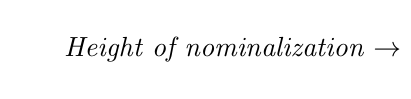
\begin{tikzpicture}
\tikzset{level distance=22pt,sibling distance=10pt}
\tikzset{level 2/.style={sibling distance=0pt}}
 \Tree [.PossP [.AspP [.VoiceP \qroof{Subject}.DP [.Voice$^\prime$  [.vP \qroof{...}.VP [.v\\{\scshape acc} ] ]  [.Voice\\{i$\varphi$: val$_{\textsc{ag}}$} ] ] ] [.Asp ]] [.Poss ] ]
 \node (c) at (-5.25,-1.05) {{\itshape  Height of nominalization $\rightarrow$}};
   \end{tikzpicture}
\end{figure}

The presence of AspP in the structure again predicts that functional restructuring should be possible in gerunds. This prediction is borne out, as shown with the aspectual suffixes `start' and `finish' in (\ref{haninkshould}--\ref{haninkfinishread}), respectively:


\ea Gerunds with restructuring \label{haninkgerundr}
\ea\gll $[$ mé:hu šáwlamhu wagay-áŋa\textit{-gáŋaʔ} $]$ k-éʔ-i\\ 
$[$ boy girl 3.talk-{\scshape appl}{\itshape-start} $]$ 3-be-{\scshape ind}\\
\glt `The boy should start talking to the girl.'\\(Lit. `The boy's starting to talk to the girl should be.') \label{haninkshould}
\ex \label{haninkfinishread}
\gll $[$ di-bamušéʔeš\textit{-mámaʔ} $]$  di-gaʔlám-i\\
$[$ 1-read\textit{-finish} $]$ 1/3-want-{\scshape ind}\\
\glt `I want to finish reading.' (Lit. `I want my finishing to read.')
\z
\z 

Regarding lexical restructuring, the presence of VoiceP in gerunds likewise predicts agent sharing to be possible (barring semantic anomaly), leading to the availability of lexical restructuring in gerunds. I unfortunately do not have data to test this prediction at present, and so I must leave this question to future work.


\subsection{Instrumental nominalizations}

Another nominalization type for which restructuring remains to be tested are instrumental nominalizations, formed by the prefix {\itshape ʔit-} (\ref{haninkinst}). As demonstrated through the availability of direct objects (\ref{haninkfly}), the causative morpheme (\ref{haninkfly}--\ref{haninkrouge}), and reflexive marking (\ref{haninkrouge}), such nominalizations target at least VoiceP.
 
\ea Instrumental nominalizations\label{haninkinst}\\
\ea \gll pú:t'eʔ ʔit-yúli-ha\\
fly {\scshape inst}-to.die-{\scshape caus}\\
\glt `fly swatter' (Lit. `something to kill flies with') \hfill Washo Archive \label{haninkfly}
\ex \gll ʔit-gum-p'áʔlu-šóšoŋ-ha\\
{\scshape inst-refl}-on.cheeks-be.red-{\scshape caus}\\
\glt `rouge'   (Lit. `something to make one's cheeks red with')\newline\phantom{x}\hfill Washo Archive \label{haninkrouge}
\z
\z
 
Due to the presence of VoiceP, it is predicted that lexical restructuring should be possible; functional restructuring is predicted to be allowed should it turn out that aspectual suffixes are also permitted. Here again I must test these predictions in future work. I note as well that an interesting case would be a type of nominalization with an intermediate size, smaller than VoiceP but larger than a root nominalization. I am unfortunately unaware of any such nominalizations in Washo, but this points to an  open empirical question for cross-linguistic research. 

 \section{Conclusion}
 
 %In this paper I have offered a preliminary overview of restructuring and nominlization in Washo, paying particular attention to  the  interaction between restructuring and nominalization size. Supporting the proposal put forward in \citet{wurmbrandshimamura2017}, I have shown that restructuring is only possible in a nominalization if that nominalization projects at least to the level of  VoiceP. As a result, restructuring is possible in thematic subject nominalizations and gerunds, but not in unexpressed theme nominalizations.
 


 Susi Wurmbrand's rich work over the years has opened to the door to many fascinating questions about the way that restructuring manifests cross-linguistically. While I have only scratched  the surface of this topic, I hope to have demonstrated that examining the interaction between restructuring and nominalization cross-linguistically is a useful tool for understanding both of these constructions.



\section*{Acknowledgments}
I would like to thank Adele James, Melba Rakow, and Ramona Dick\textsuperscript{†}, who have patiently worked with me over the years on the Washo language. I also thank Karlos Arregi, Andrew Koontz-Garboden, and the audience at GLOW 43 for helpful discussion of various aspects of the ideas presented here, as well as the two anonymous reviewers of this paper. All errors and shortcomings are my own.



\section*{Abbreviations}
\begin{tabularx}{.5\textwidth}{@{}lQ}
{\scshape acc} & accusative\\
{\scshape attr} & attributive\\ 
{\scshape appl} & applicative\\
{\scshape caus} & causative\\
{\scshape dep} & dependent mood\\
{\scshape ds} & different subject (switch reference)\\
{\scshape in} & intransitive \\
{\scshape incl} & inclusive\\
{\scshape ind} & independent mood\\
{\scshape inst} & instrumental nominalizer\\
{\scshape neg} & negation\\
\end{tabularx}%
\begin{tabularx}{.5\textwidth}{lQ@{}}
 {\scshape nm} & clausal nominalizer\\
 {\scshape nmlz} & nominalizer\\
 {\scshape pl} & plural\\
 {\scshape prog} & progressive\\
 {\scshape prosp} & prospective aspect\\
 {\scshape rec.pst} & recent past\\
 {\scshape refl} & reflexive\\
 {\scshape ss} & same subject\\
 {\scshape stat} & static\\
 {\scshape tr} & transitive\\
 {\scshape un} & unexpressed possessor agreement\\
\end{tabularx}

{\sloppy\printbibliography[heading=subbibliography,notkeyword=this]}

\end{document}
